\documentclass{article}
\usepackage[utf8]{inputenc}

\title{Chem132A Discussion 3 Homework}
\author{Moises Romero (moiseser@uci.edu), Shane Flynn (swflynn@uci.edu) }
\date{10/15/17}


\usepackage{graphicx}
\usepackage{amsmath}
\usepackage{braket}
\usepackage[margin=0.7in]{geometry}


\newcommand{\be}{\begin{equation}}
\newcommand{\ee}{\end{equation}}
\newcommand{\pd}{\partial}

\begin{document}

\maketitle

\section{Entropy is a State Function}
Entropy can be used to describes the disorder in a system. 
In class we defined the entropy to be:
\be
\Delta S \equiv \int  \frac{\delta q_{r}}{T}
\ee

If we wish to consider irreversible processes, a more general description of the Entropy would be the inequality: 
\be
\Delta S \geq \int  \frac{\delta q_{r}}{T}
\ee

Consider the following figure (it should look familiar from Discussion Problem Set 2). 
\begin{figure}[h]
\caption{Point 1: (P$_1$,V$_1$,T$_1$), Point 2: (P$_1$,V$_2$,T$_3$), Point 3: (P$_2$,V$_2$,T$_1$), Point 4: (P$_3$,V$_2$,T$_2$)}
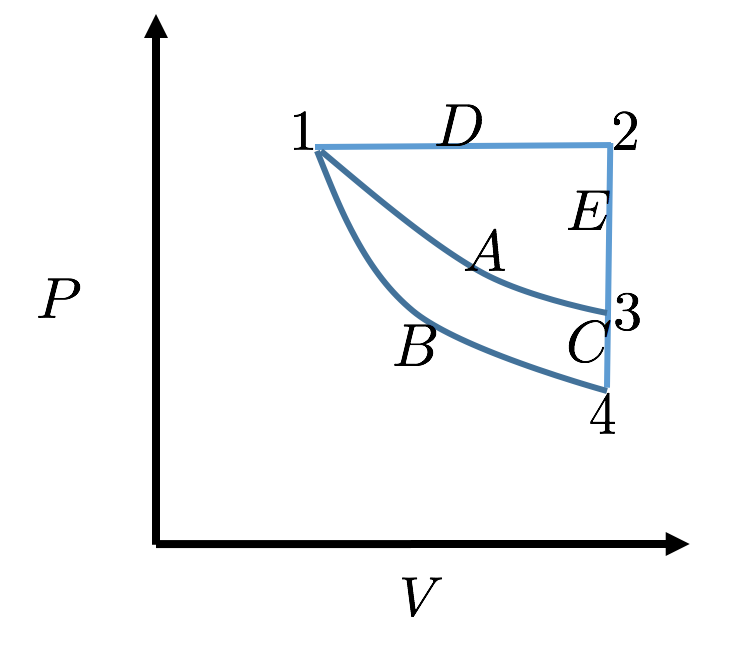
\includegraphics[width=0.5\textwidth]{cycle.png}
\end{figure}

This week we will explore the Second Law, again through the various pathways as defined in the diagram.

Consider a closed system containing 1 mole of gas. 
We will assume that the gas obeys the following Equation of State (x and y are constants). 
We will also assume that this specific gas has an internal energy that only depends on T and not V $\Rightarrow$ U(T). 
\be
\frac{P}{V}=\frac{RTx}{V}+\frac{RTy}{V}
\ee

\subsection{Pathway A}
Compute the Entropy for: 1 mole of gas traversing pathway A.
Take path A to be an isothermal expansion. 

\subsection{Pathway B+C}
Next, compute the Entropy for 1 mole of gas traversing pathways B and then C.  
Take path B to be a reversible adiabatic expansion and path C a reversible isochoric process. 

\textbf{Hint:}
For pathway B you will need to transform your integral from dT to dP to make a meaningful comparison. 
To do this consider just pathway B (the adiabatic process), is there any relationship relating dT and dP?

\subsection{Time to be Lazy}
Without doing any calculations associated with pathways D and E what can we say about the change in Entropy associated with traversing these pathways?

\subsection{Entropy of a Free Expansion}
A \textbf{Free Expansion} is an irreversible process which occurs when a gas expands into a vacuum. 
Because the gas expands into vacuum, there is no work done on/by the gas. 

A gas at T is allowed to expand from V$_1$ to an end volume of V$_2$. 
This is an irreversible process, and there is no heat transfer that occurs during the process: q$_{irr}$ = 0.

Calculate the change in Entropy associated with one mole of gas undergoing this Free Expansion. 
Again we will assume the gas follows this Equation of State:
\be
\frac{P}{V}=\frac{RTx}{V}+\frac{RTy}{V}
\ee
And that the gas has an Internal Energy that is only a function of T: U(T).

\section{Fundamental Equations}

\subsection{Internal Energy and Entropy}
Consider a closed system, with an ideal gas undergoing a reversible expansion (assume only PV work). 

\subsubsection{New Variables}
Re-write the differential form of the  First Law of Thermodynamics, by explicitly substituting in the Second Law. 
What variables do you find, that Internal Energy naturally depends on: U(?,?). 

The work-flow for the question should look something like
\be
\begin{split}
dU = \delta q + \delta w\\
dU = \delta q + -PdV\\
\cdots \\
dU = ?d? + -PdV
\end{split}
\ee

\subsubsection{Partial Derivatives}
Write a total differential for Internal Energy associated with each of these variables.
Can you relate the partial derivatives of your total differential to the differential equation from the previous section?

One of the partial derivatives you can write will be 
U(?,V)
\be
\begin{split}
dU = ? d? + \left(\frac{\pd U}{\pd V}\right)_?dV\\
\Rightarrow \left(\frac{\pd U}{\pd V}\right)_? = -P
\end{split}
\ee

\subsubsection{More Math}
Now, using the fact that Internal Energy is a State Function use these two variables to relate some partial derivatives 
\be
\left(\frac{\pd ^2 U}{\pd ? \pd ?}\right)_? = ?
\ee

\subsection{Enthalpy and The First 2 Laws}

\subsubsection{The Fundamental Equation}
Using your result from the previous problem, please determine the two natural variables associated with the Enthalpy when considering the First and Second Law: H(?,?).

\textbf{Comment:} 
Start with your definition of Enthalpy, and substitute the equation you found for dU from above. 

\subsubsection{The Total Differential}
Write a total differential associated with each of these variables.
Can you relate the partial derivatives of your total differential to the differential equation?

\subsubsection{Computing Your Maxwell}
Now take the second derivative of H to relate some partial derivatives. 

\subsection{Helmholtz and The First 2 Laws}

\subsubsection{The Fundamental Equation}
Using the definition of the Helmholtz Free Energy determine the two natural variables associated with the Helmholtz (with the same process as above): A(?,?)

\subsubsection{The Total Differential}
Write a total differential associated with each of these variables.
Can you relate the partial derivatives of your total differential to the differential equation?

\subsubsection{Computing Your Maxwell}
Now take the second derivative of A to relate some partial derivatives.

\subsection{Gibbs as a Double Transformation}

\subsubsection{The Fundamental}
Using the definition of the Gibbs Free Energy determine the two natural variables associated with the Gibbs Free Energy: G(?,?)

\subsubsection{The Total Dif.}
Write a total differential associated with each of these variables.
Can you relate the partial derivatives of your total differential to the differential equation?

\subsubsection{Computing Your Maxwell}
Now take the second derivative of G to relate some partial derivatives.

\section{Time to Type}
The exam is just around the corner. 
Spend this week to start studying for the exam. 
Try working through your notes and the textbook to type up a formal study guide for the course. 
Think about including key definitions and their meaning, key equations and their conditions for being true, and highlight any sections of the course that you did not understand the first time around. 

Any conceptual topics (and associated problems) that were particularly difficult should be revisited before the exam! 

\end{document}